\begin{itemize}
	
\item \textbf{Save User Route:}\\Coding standards were upheld and the code was well documented. However, the lack of compartmentalization of functionality may prove problematic when  removing, adding, or editing program features. Furthermore, the location data is kept in a single file with the program therefore if a location should be added it cannot be added with a database query but had to be done manually.\\
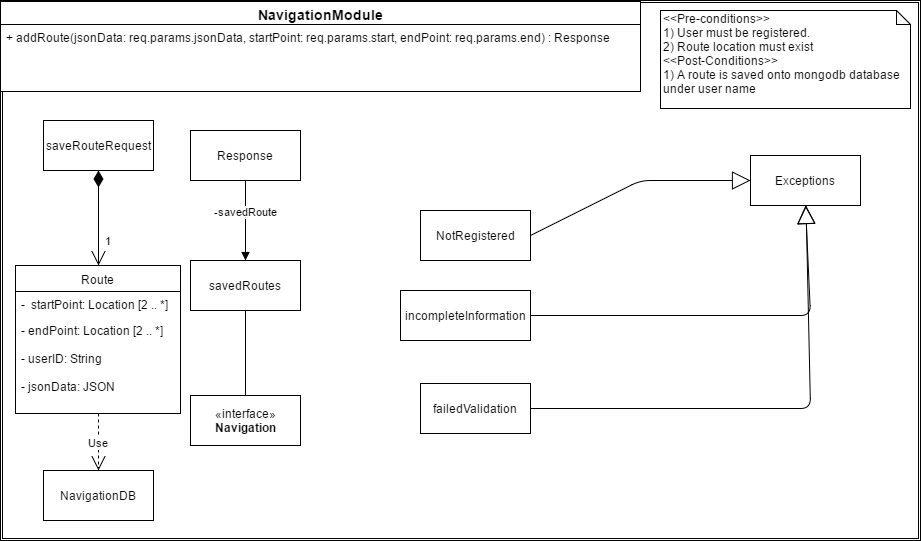
\includegraphics[scale=0.5]{SaveRoute.png}
\caption{Service Contract: Save User Preference}
	\textbf{Mark: 6/10}
\item \textbf{Save User Preference:}\\MongoDB as a choice of database management is favourable especially with regards scalability. However, the location data is not stored in a MongoDB database but rather in the same navigationLocal.js file as the entire program. This will cause a bottleneck when the amount of location data is increased.\\
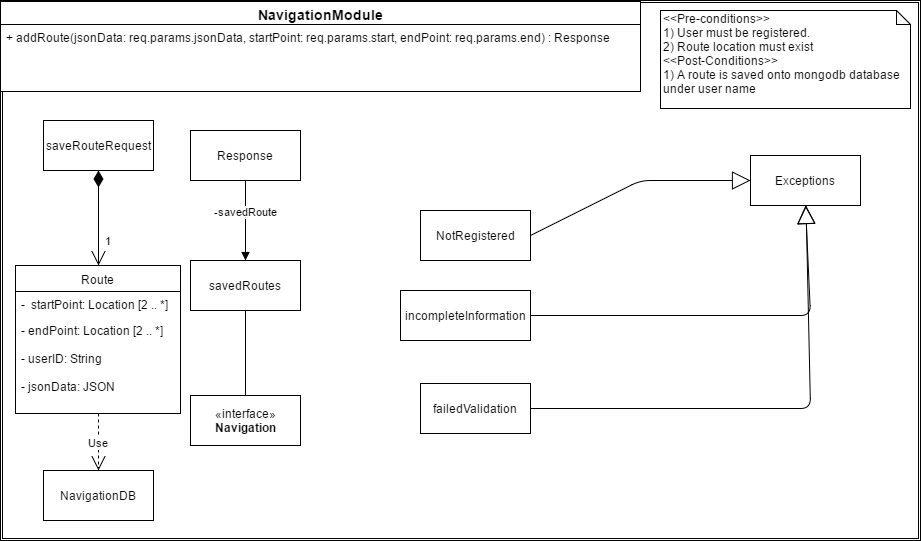
\includegraphics[scale=0.5]{SaveRoute.png}
\caption{Service Contract: Save User Preference}
	\textbf{Mark: 7/10}
\item \textbf{Cache Routes:}\\MongoDB as a choice of database management is favourable especially with regards scalability. However, the location data is not stored in a MongoDB database but rather in the same navigationLocal.js file as the entire program. This will cause a bottleneck when the amount of location data is increased.\\
	\textbf{Mark: 7/10}
	
\end{itemize}